\section{FSM con flip-flops en estilo \textit{One-Hot} modificado \label{sec:s2}}

\begin{center}
	\begin{minipage}{12cm}
		\begin{tcolorbox}[title=Actividad 2]
			Considerar la tabla ``\textit{ONE – HOT} modificada'':\enter
			
				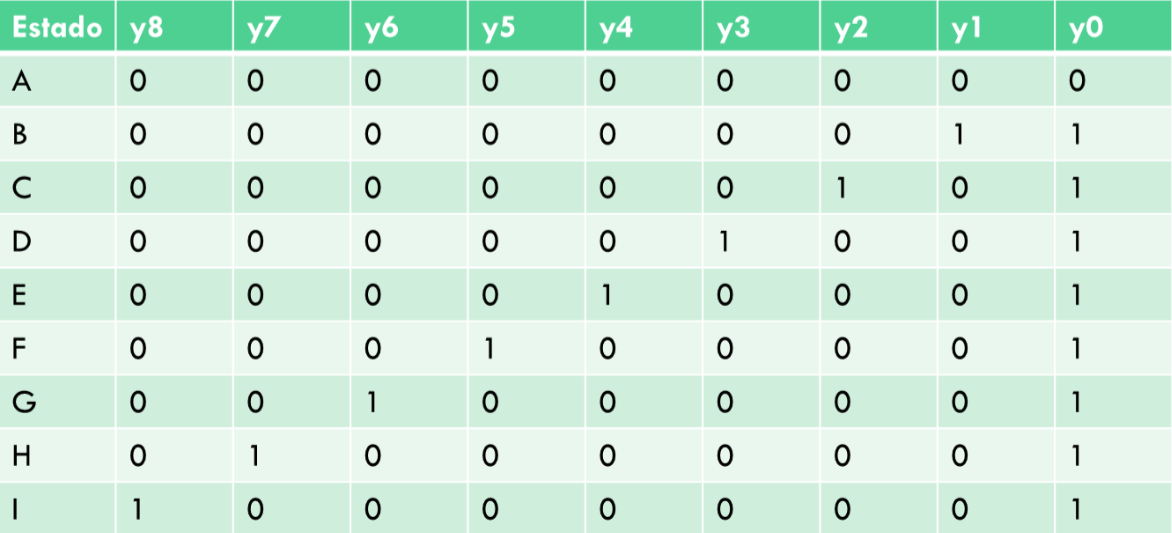
\includegraphics[scale=0.3,center]{OneHotModified.png}
			Diseñar utilizando las ecuaciones de los flip-flops de la tabla modificada. Observar el resultado en el visor RTL. Compilar y simular.
		\end{tcolorbox}	
	\end{minipage}
\end{center}

La visualización RTL de la FSM, descrita en estilo \textit{One-Hot} modificado, se muestra en la \autoref{fig:FSM_OneHotM_RTL}. La implementación en hardware utiliza a los 9 flip-flops descritos en el código y los interconecta de acuerdo a la ecuaciones descritas, haciendo uso de múltiples compuertas lógicas. Las simulaciones se visualizan en la \autoref{fig:FSM_OneHotM_Wave}. Se observa que primero detecta 4 ceros consecutivos y pone en alto a S, aunque W inicia con ``01''. Después de restablecer el sistema (utilizando a RST), la FSM detecta 4 unos consecutivos y pone nuevamente en alto a S, para después volver a ponerla en bajo, ya que la secuencia continúa con ``01''.

En los Anexos se localiza la descripción de la FSM con estilo \textit{One-Hot} modificado. Además de las entradas y salida, se declararon 9 flip-flops y con una lista sensible a los flancos de subida de CLK y de bajada de RST, se describió el comportamiento de cada flip-flop, de acuerdo a su ecuación obtenida. Al momento de restablecer el sistema, se inicializa a cada flip-flop, tomando el estilo \textit{One-Hot} modificado. En comparación con la Actividad 1, el circuito tiene el mismo funcionamiento e implementa la misma cantidad de flip-flops, unicamente cambia el estilo de codificación alterando un poco las ecuaciones del estilo original.

\begin{figure}[ht]
	\centering
	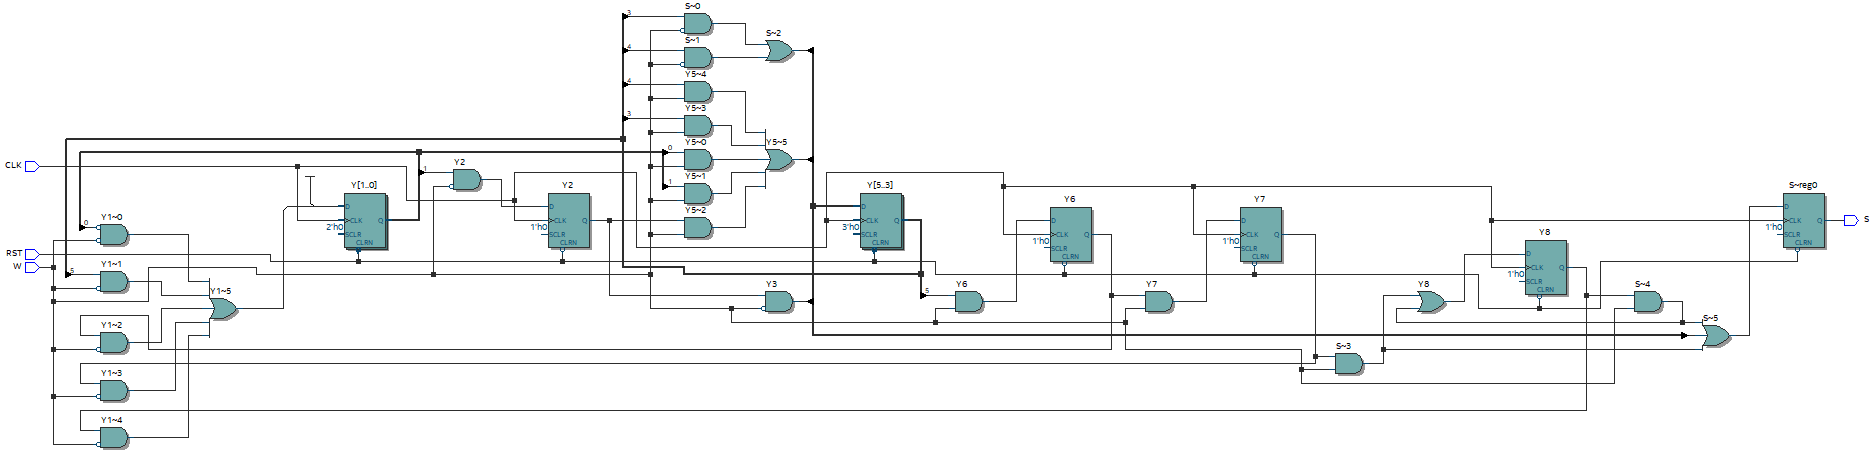
\includegraphics[scale=0.34]{FSM_OneHotM_RTL.png}
	\caption{Diagrama RTL de la FSM, descrita con las ecuaciones de los flip-flops codificados en \textit{One-Hot} modificado. \label{fig:FSM_OneHotM_RTL}}
\end{figure}

\begin{figure}[ht]
	\centering
	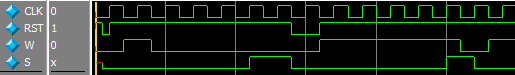
\includegraphics[scale=1.2]{FSM_OneHot_Wave.png}
	\caption{Simulación de la FSM, descrita con las ecuaciones de los flip-flops codificados en \textit{One-Hot} modificado, en el visor de formas de onda de ModelSim. \label{fig:FSM_OneHotM_Wave}}
\end{figure}